\begin{frame}{Foundations: Access Structures}
	\begin{itemize}
		\item Parties: \(\mathcal{P} = \{P_1,\dots,P_n\}\).
		\item Access structure \(\mathcal{A}\subseteq 2^{\mathcal{P}}\): subsets that can reconstruct.
		\item \textbf{Monotone} requirement: if \(A\in\mathcal{A}\) and \(A\subseteq B\), then \(B\in\mathcal{A}\) \cite{beimel2011secret}.
	\end{itemize}

	\textbf{\textcolor{blue}{Examples}}
	\begin{itemize}
		\item Threshold: "any \(t\) out of \(n\)".
		\item Boolean policy: \((\text{CEO} \wedge \text{CFO}) \vee (\text{2 of 3 managers})\).
		\item Compartmented / hierarchical policies (common in organizations).
	\end{itemize}

	\begin{figure}
		\centering
		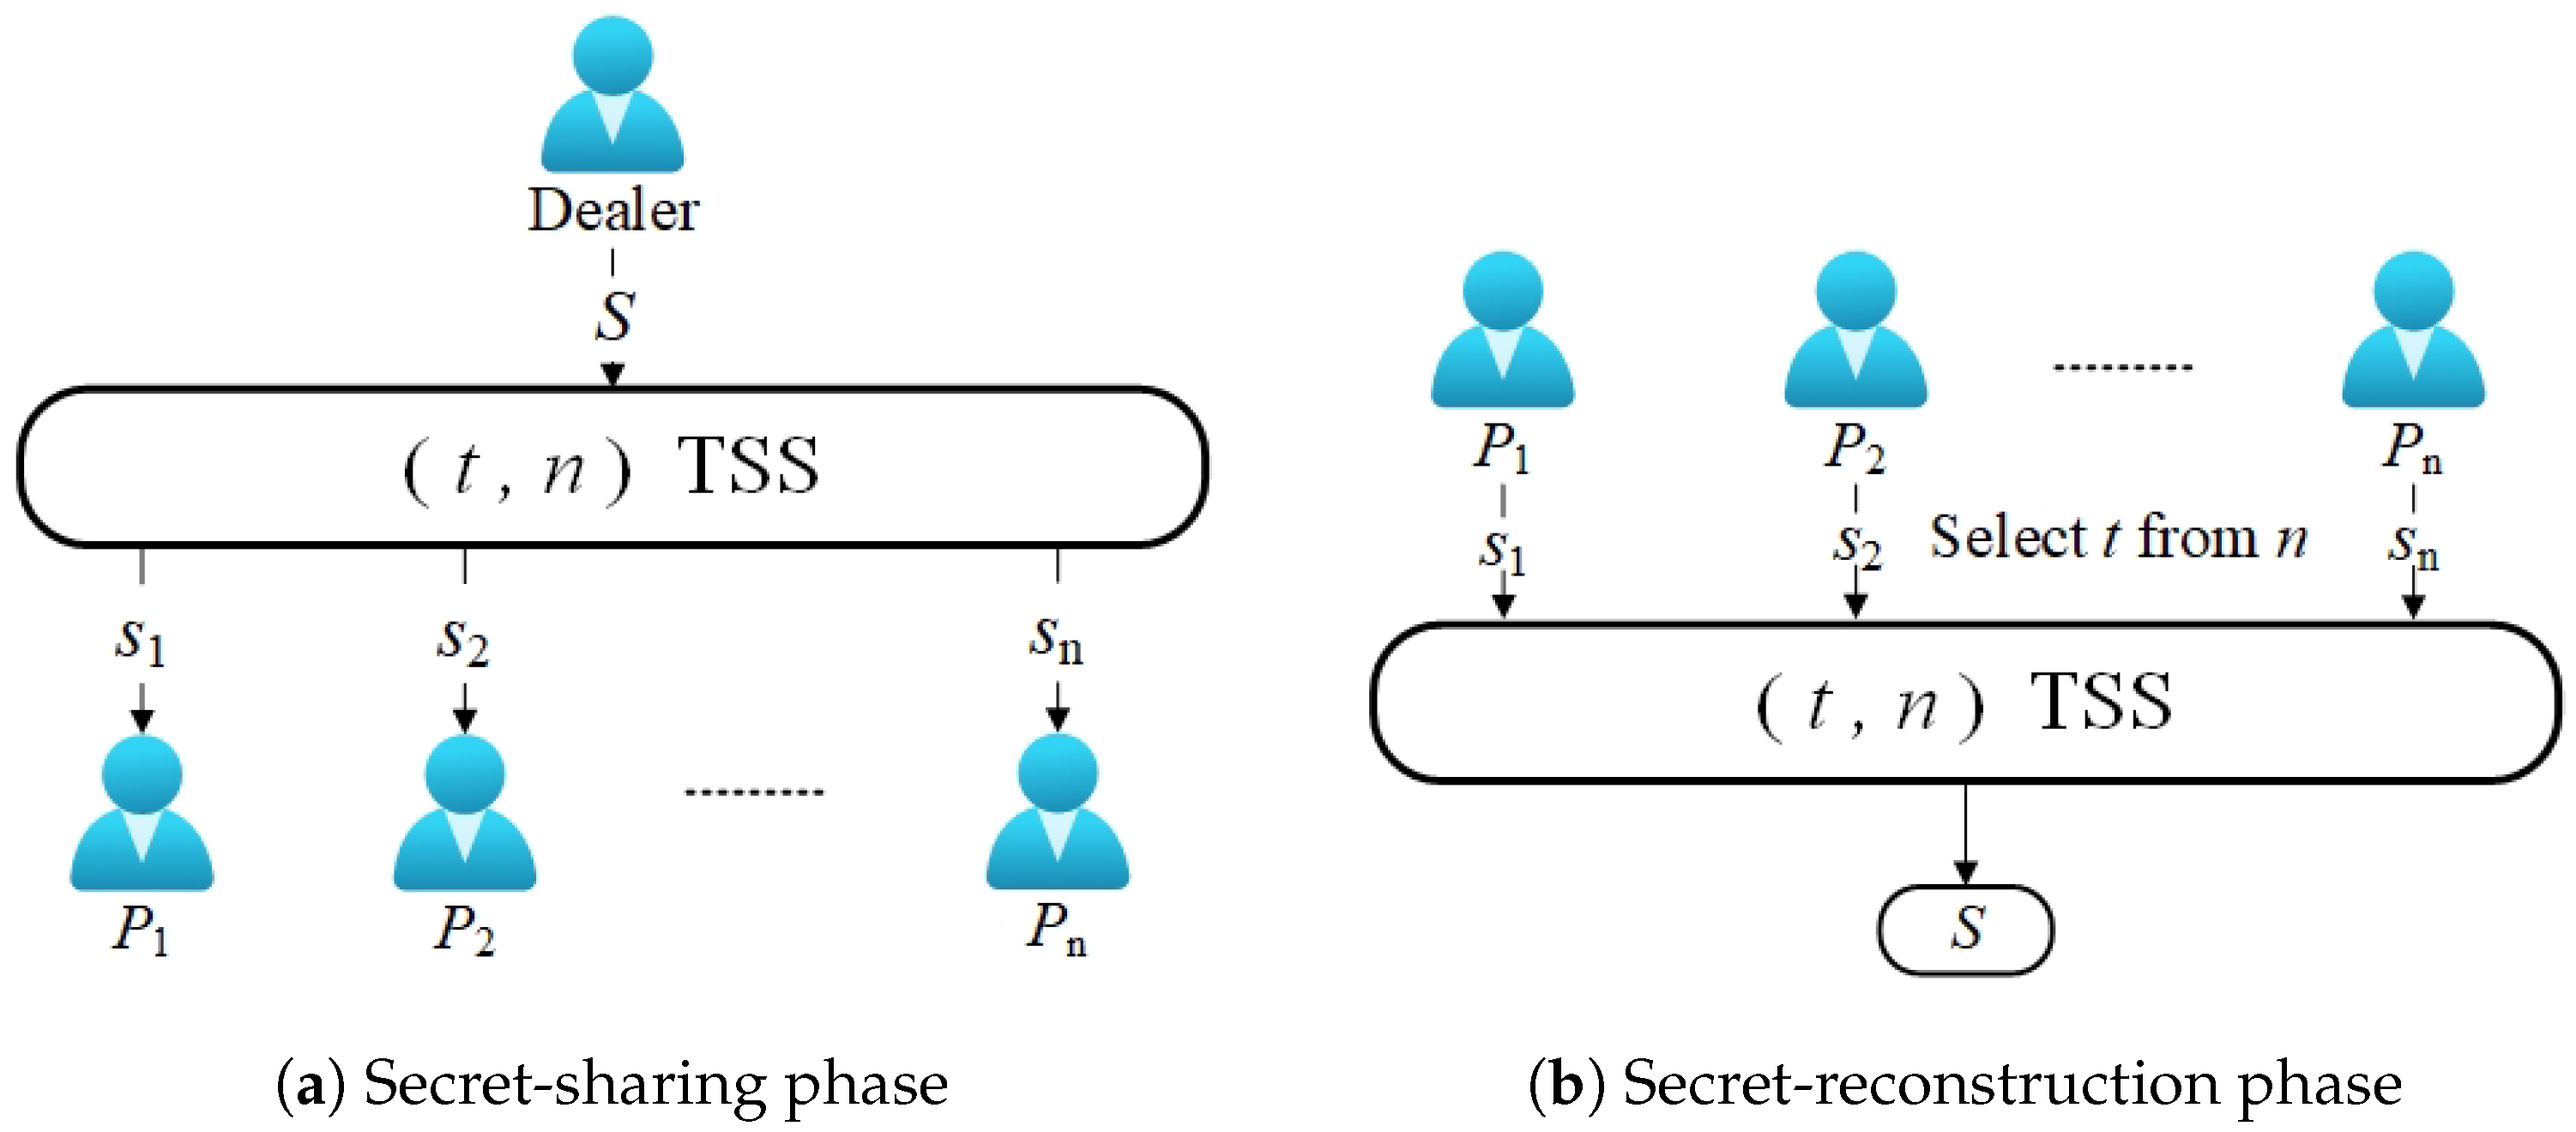
\includegraphics[scale=0.5]{fig/fig-secret-sharing-phases.png}
		\caption{Secret Sharing Scheme Phases}
	\end{figure}
\end{frame}

\begin{frame}{Security Definitions and Metrics \cite{beimel2011secret}}
	Let secret \(S\) be random and shares be random variables \(\{S_i\}\). A scheme realizing \(\mathcal{A}\) satisfies:
	\begin{itemize}
		\item \textbf{Correctness:} for every \(A\in\mathcal{A}\), \(S\) is determined by \(\{S_i : P_i\in A\}\).
		\item \textbf{Perfect privacy:} for every \(T\notin\mathcal{A}\), shares reveal no information:
		\[
			I(S;\{S_i: P_i\in T\}) = 0
			\quad\Longleftrightarrow\quad
			H(S\mid \{S_i: i\in T\}) = H(S).
		\]
	\end{itemize}

	\textbf{\textcolor{blue}{Efficiency metrics}}
	\begin{itemize}
		\item \textbf{Information rate}: share size vs secret size (ideal if equal).
		\item \textbf{Computation}: sharing + reconstruction complexity.
		\item \textbf{Robustness/verifiability}: tolerate or detect cheating.
	\end{itemize}
\vspace{0.2cm}
	\textbf{\textcolor{blue}{Context: ideality}}
	\begin{itemize}
		\item \textbf{Ideal scheme}: share size equals secret size.
		\item Threshold structures are ideal; some non-threshold structures also are \cite{brickell1989some}.
	\end{itemize}
\end{frame}
